\documentclass[11pt,a4paper]{scrartcl}
\usepackage[ngerman]{babel}
\usepackage[utf8]{inputenc}
\usepackage[T1]{fontenc}
\usepackage{graphicx}
\usepackage{float}
\usepackage{fullpage}
\usepackage{amssymb}
\usepackage{url}                % URLs
\usepackage{tikz}               % for the grey border on the title page
\usepackage[absolute,overlay]{textpos}

\usepackage[a4paper,left=40mm,right=30mm,top=20mm,bottom=20mm,includeheadfoot]{geometry}
\newcommand{\changefont}[3]{\fontfamily{#1} \fontseries{#2} \fontshape{#3} \selectfont}
\parindent 0pt
\usepackage[raiselinks=true,
						bookmarks=true,
						bookmarksopenlevel=1,
						bookmarksopen=true,
						bookmarksnumbered=true,
						hyperindex=true,
						plainpages=false,
						pdfpagelabels=true,
						pdfborder={0 0 0.5},
						colorlinks=false,
						linkbordercolor={0 0.61 0.50},
						citebordercolor={0 0.61 0.50}]{hyperref}  %{0.57 0.74 0.57}

\author{PSE-Projekt 4 Team 2}
\title{Pflichtenheft zu Worthwhile}

\setcounter{tocdepth}{1} % make TOC fit on one page

\hyphenation{Worth-while}

\newcommand{\reqtype}{}
\newenvironment{reqlist}[1]{\begin{description} \renewcommand{\reqtype}{#1}}{\end{description}}
\newcommand{\req}[3]{\item[\textbf{/\reqtype{}#1/}] #2 \\ #3}
\newcommand{\see}{\ensuremath{\rightarrow}}

\newcommand{\testspec}[4]{
		\begin{description}
			\item[Testziel] #1
			\item[Vorbedingungen] #2
			\item[Beschreibung] #3
			\item[Ergebnis] #4
		\end{description}}

\graphicspath{{images/}}

\begin{document}

%% titlepage.tex
%%

% coordinates for the bg shape on the titlepage
\newcommand{\diameter}{20}
\newcommand{\xone}{-30}
\newcommand{\xtwo}{150}
\newcommand{\yone}{15}
\newcommand{\ytwo}{-265}

\begin{titlepage}
% bg shape
\begin{tikzpicture}[overlay]
\draw[color=gray]
 		 (\xone mm, \yone mm)
  -- (\xtwo mm, \yone mm)
 arc (90:0:\diameter pt)
  -- (\xtwo mm + \diameter pt , \ytwo mm)
	-- (\xone mm + \diameter pt , \ytwo mm)
 arc (270:180:\diameter pt)
	-- (\xone mm, \yone mm);
\end{tikzpicture}

	\begin{textblock}{10}[0,0](1.7,1)
		
\includegraphics[width=.3\textwidth]{images/kit_logo_de_4c_positiv.pdf}
	\end{textblock}
	\changefont{phv}{m}{n}	% helvetica	
	\begin{center}
		\fontsize{45}{50}\selectfont
        \vfill
        \textsc{Worthwhile} \\
        \textsc{Pflichtenheft}
        \vfill
		\LARGE
		PSE WS 11/12
  \vfill
 \newpage
 
 \null
 \vfill
 
 Praxis der Softwareentwicklung -- WS 2011/2010 \\
  Automatisches Prüfen der Korrektheit von Programmen \\
  Projekt 4 -- Gruppe 2 \\
  \medskip
  \vspace{2cm}
  \Large
  \begin{tabular}{|l|l|}
    \hline
    Leon Handreke & 123456 \\
    \hline
    Chris Hiatt & 1610922 \\
    \hline
    Stefan Orf & 123456 \\
    \hline
    Joachim Priesner & 1579308 \\
    \hline
    Fabian Ruch & 123456 \\
    \hline
    Matthias Wagner & 1579342 \\
    \hline
  \end{tabular}
  \vspace{2cm} \\
  \today \\
	Revision 0
	\end{center}
	
  \vfill

\end{titlepage}


\tableofcontents
\clearpage

\section{Einleitung}

\subsection{Arbeitsweise während der Implementierungsphase}
\begin{frame}
\frametitle{Die Arbeitsweise während der Implementierungsphase}

\begin{itemize}
	\item<+-> Ausnutzung der Verfügbarkeit hilfreicher Werkzeuge wie Bug-Tracker, Code-Review, Continuous-Integration mit automatischen Tests und statischer Analyse
	\item<+-> AST-Attrappenerstellung für Testprogramme
	\item<+-> Parallele Komponentenentwicklung
	\item<+-> Regelmäßige Treffen
\end{itemize}
\end{frame}

\subsection{Zeitlicher Ablauf}
\begin{frame}
\frametitle{Zeitlicher Ablauf}

\begin{figure}
	\vspace{-0.15cm}
	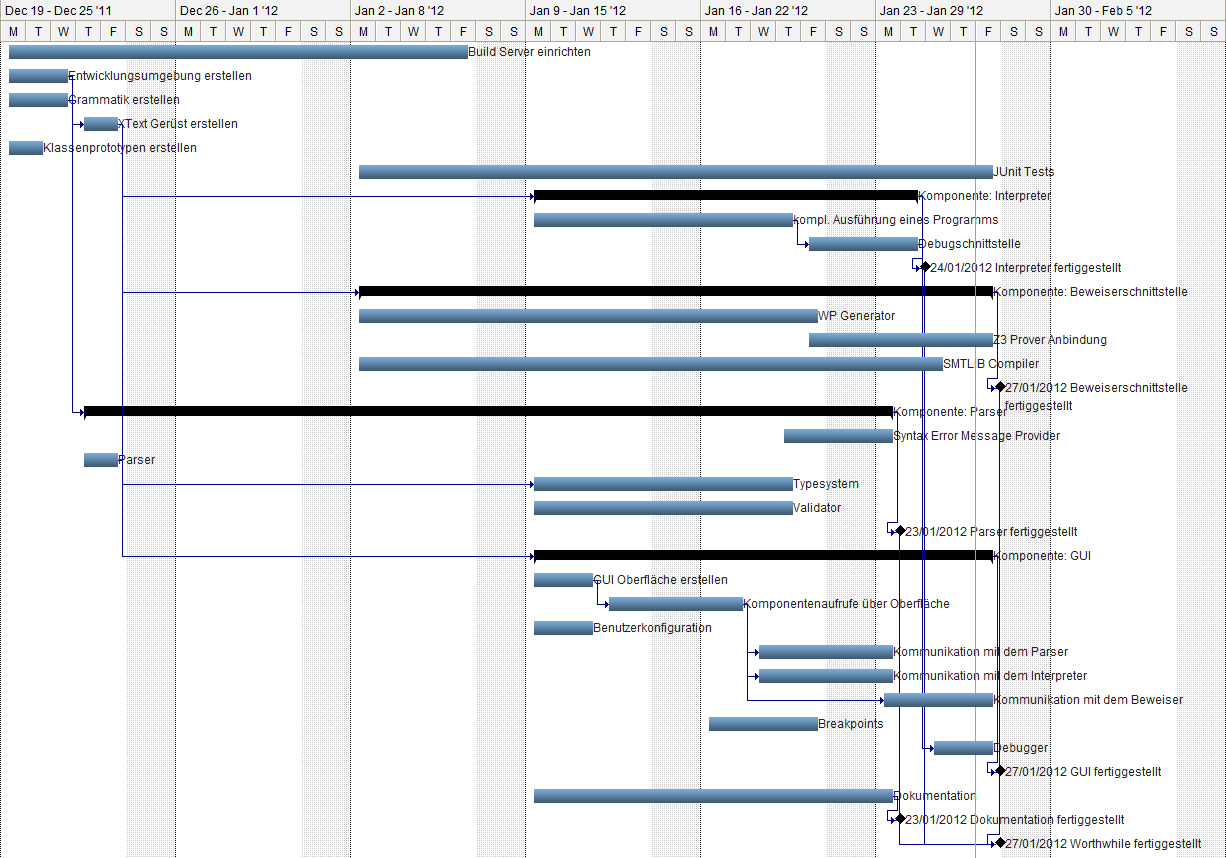
\includegraphics[height=0.95\textheight]{../bericht/images/gantt_implementierung_diag.png}
\end{figure}
\end{frame}

\subsection{Section}
\begin{frame}
\frametitle{Frametitle}

\end{frame}


\section{Produkt"ubersicht}%

\textit{Worthwhile} ist ein m"achtiges Analysewerkzeug f"ur eine einfache WHILE-""Programmiersprache. Bei der Programmanalyse kommen dabei sowohl klassische Techniken der Laufzeitanalyse (interaktives Debuggen, Überprüfung von Zusicherungen zur Laufzeit) als auch moderne, logikbasierte Methoden der Softwareverifikation zum Einsatz.\footnote{Quelle: Projektspezifikation unter \url{http://formal.iti.kit.edu/teaching/pse/2011/}} \textit{Worthwhile} vereinigt s"amtliche Arbeitsschritte von der Programmerstellung bis zur Programmverifikation unter einer einzigen komfortablen und leicht benutzbaren Oberfl"ache. Außerdem ist \textit{Worthwhile} Ausführungsumgebung für die entwickelten WHILE-""Programme.%

\subsection{Anwendungsfall-""Übersicht}

Im folgenden Anwendungsfalldiagramm sind die unterschiedlichen Möglichkeiten zur Benutzung des Systems dargestellt:

\begin{figure}[H]
	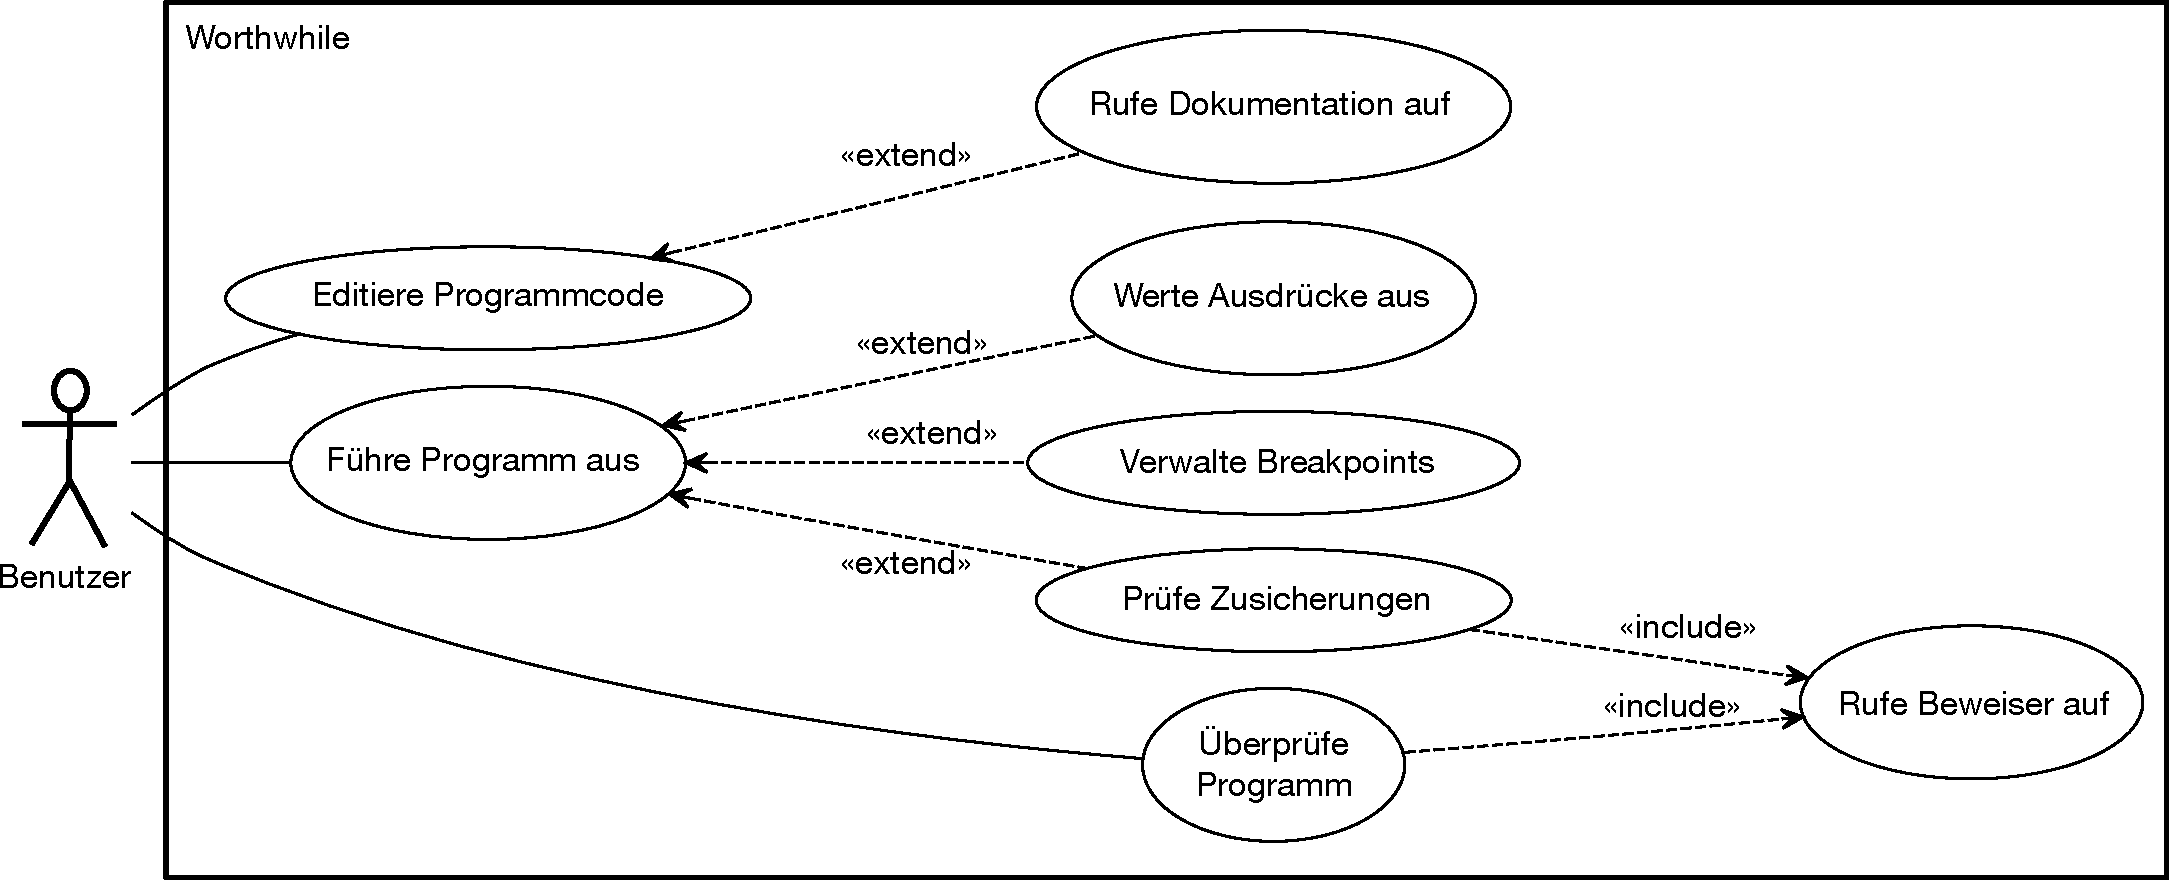
\includegraphics[width=\textwidth]{usecase/usecase.pdf}
\end{figure}


\section{Zielbestimmung}%

% TODO Nachverfolgbarkeit der Anforderungen: Jeder funktionalen Anforderung muss eine Zielbestimmung zuzuordnen sein $\Rightarrow$ evtl. Zielbestimmungen ergänzen

\subsection{Interpreter}%

Der \see{Interpreter} ermöglicht die (schrittweise) Ausführung eines Programms und die Inspektion des aktuellen Programmzustands durch den Benutzer.%

\begin{description}%
    \item[Wunsch] Der Benutzer kann den Programmzustand w"ahrend der Ausf"uhrung "andern.%
    \item[Wunsch] Während eines Programmdurchlaufs können benutzerdefinierte Ausdr"ucke "uber dem Programmzustand ausgewertet werden.%
\end{description}%

\subsection{Run-time-""Checker}%

Der \see{Run-time-""Checker} erlaubt die Pr"ufung von \see{Zusicherungen} in Programmen f"ur einen konkreten Programmdurchlauf, d.~h.\ zur Laufzeit.%

\begin{description}%
    \item [Muss] Die im Programm eingebetteten (quantorenfreien) \see{Annotationen} werden ausgewertet. Im Fehlerfall erfolgt die Rückmeldung "uber die grafische Benutzeroberfl"ache.
    \item [Soll] Eingebettete Formeln mit Quantoren "uber einem eingeschr"ankten Bereich werden ausgewertet.%
    \item [Wunsch] Eingebettete Formeln mit Quantoren über uneingeschränkten Bereichen werden mit Hilfe eines \see{Beweisers} ausgewertet.
\end{description}%

\subsection{Grafische Benutzeroberfl"ache}%

Die grafische Benutzeroberfl"ache dient zur Steuerung der einzelnen Komponenten des Systems sowie der Anzeige von R"uckmeldungen der (externen) Module des Werkzeugs.%

\begin{description}%
    \item [Muss] Die Sprache der Benutzeroberfläche ist Englisch.%
    \item [Abgrenzung] Die Benutzeroberfläche enthält nur Optionen und Funktionen, die der besseren oder einfacheren Eingabe und Analyse eines Programms durch den Benutzer zutr"aglich sind.%
    \item [Wunsch] Es werden zur besseren Lesbarkeit Unicode-""Symbole f"ur logische Operatoren und Quantoren angezeigt.%
\end{description}%

\subsection{WHILE-""Sprache}%

Die vom \textit{Worthwhile}-""Interpreter erkannte Programmiersprache ist eine \see{WHILE-""Sprache}.

\begin{description}%
    \item [Muss] Grundlegende Sprachkonstrukte: \texttt{if}-""Anweisungen und \texttt{while}-""Schleifen
    \item [Muss] Variablen mit Ganzzahlen~(\texttt{Integer}), Wahrheitswerten~(\texttt{Boolean}) sowie Arrays von \texttt{Integer} und \texttt{Boolean} als Datentypen%
    \item [Wunsch] Definition und Aufruf von eigenen Funktionen%
    \item [Abgrenzung] Weder Strings, Gleitkommazahlen, Zeiger noch eigene Datentypen%
    \item [Abgrenzung] Kein Heap%
    \item [Abgrenzung] Keine Nebenl"aufigkeit%
\end{description}%

\subsection{Annotationssprache}%

In der \see{Annotationssprache} werden die vom Beweiser gepr"uften WHILE-""Programme spezifiziert und die Zusicherungen für den Run-time-""Checker formuliert.%

\begin{description}%
    \item [Muss] Annotationen sind im Quelltext des Programms eingebettet, aber durch spezielle Syntax klar vom Programm getrennt.%
    \item [Muss] Syntax und Semantik von Ausdr"ucken werden, soweit m"oglich, aus der Programmiersprache "ubernommen.%
    \item [Muss] Grundlegende Annotationen: Zusicherungen (Assertions) und Annahmen (Assumptions)%
    \item [Muss] Annotationen erlauben Aussagen der \see{Prädikatenlogik} "uber den Zustand einer Programmausf"uhrung.%
    \item [Soll] Spezielle Syntax~("`syntactic sugar"'), um die Verst"andlichkeit von Annotationen zu verbessern und ihre Formulierung intuitiver zu gestalten:%
        \begin{itemize}%
            \item Vor- und Nachbedingungen an Funktionen%
            \item Invarianten an Schleifen%
            \item Globale Annahmen in Programmspezifikationen%
        \end{itemize}%
    \item [Wunsch] M"oglichkeit, mehrere Vor- und Nachbedingungen f"ur eine Funktion anzugeben%
\end{description}%

\subsection{Beweiserschnittstelle}%

Die Schnittstelle zwischen \textit{Worthwhile} und dem Beweiser ist zuständig für die Formulierung der Behauptung, dass ein Programm seine Spezifikation erfüllt, als Eingabe für den Beweiser. Außerdem muss sie bei einem Spezifikationsfehler den gescheiterten Beweisversuch, welcher vom Beweiser als Ausgabe geliefert wird, als Gegenbeispiel formulieren. Nicht erfolgreiche Beweisversuche können sowohl Folge unzureichender Annahmen als auch fehlerhafter Implementierungen sein.%

\begin{description}%
    \item [Muss] Übersetzung eines Programms und seiner Spezifikation in eine vom Beweiser überprüfbare prädikatenlogische Formel
    \item [Muss] Übersetzung von Modellen, welche der Beweiser für die Nichterfülltheit einer Spezifikation liefert, in Aufrufe des spezifizierten WHILE-""Programms%
    \item [Muss] Aufrufen des Beweisers
    \item [Muss] Behandlung von Fehlermeldungen des Beweisers, welche die prädikatenlogische Übersetzung einer Spezifikation betreffen%
    \item [Abgrenzung] Keine automatische Findung von Schleifeninvarianten
\end{description}%

\subsection{Dokumentation und Beispielsammlung}%

\begin{description}%
    \item [Muss] Dokumentation f"ur die verwendete Programmier- und Annotationssprache%
    \item [Muss] Mitgelieferte Sammlung von kommentierten und spezifizierten Beispielprogrammen zur Verdeutlichung der Funktionalit"at von \textit{Worthwhile}%
\end{description}%


\section{Produkteinsatz}%

\subsection{Anwendungsbereich}%

Die Anwendung dient zur Analyse und Verifikation von Programmen und soll Anwendern speziell im Kontext der Forschung und Lehre die M"oglichkeit geben, schnell eigene Ideen in eine Programmiersprache zu fassen und mit einem \see{Beweiser} zu analysieren.%

Außerdem dient die Anwendung als Schnittstelle im interaktiven Prozess zwischen Benutzer und Beweiser, der entsteht, wenn die Überprüfung der Programm- bzw. Funktionsspezifikation durch den Beweiser fehlschlägt und die Spezifikation (bei korrekter Implementierung) angepasst werden muss. Dies führt schließlich zur einer verifizierbaren Spezifikation und gleichzeitig zu einem besseren Verständnis des Entwicklers, was das Programm bzw. eine Funktion bewiesenermaßen tut. Nicht zuletzt liefert die Menge der Spezifikationen eine gute Dokumentation von Programmierschnittstellen.%

\subsection{Zielgruppe}%

Die Anwendung soll von Lernenden sowie Lehrenden im Umfeld einer Lehreinrichtung (z.~B.\ Besucher von Einf"uhrungsveranstaltungen in die Programmverifikation) verwendet werden. Entsprechend kann man Kenntnis von anderen Programmiersprachen sowie Vertrautheit mit Grundkonzepten der Programmverifikation (z.~B.\ der Beschreibung eines Programmzustandes mit Quantoren) voraussetzen.%

\subsection{Betriebsbedingungen}%



\section{Produktumgebung}%

\subsection{Software}%

\begin{description}%
    \item [Betriebssystem] \see Windows oder \see Linux%
    \item [\see Java Runtime Environment] Version 1.6 oder h"oher%
    \item [\see Z3] 3.2%
\end{description}%

\section{Hardware}%

\textbf{TODO:} Hardware-Anforderungen bestimmt durch Eclipse und Z3, herausfinden und hier eintragen%

\section{\see Orgware}%

Entfällt.%

\section{Schnittstellen}%

\begin{description}%
    \item [\see Eclipse Platform]%
\end{description}%



\section{Funktionale Anforderungen}
\subsection{GUI}

\subsubsection{Editor-Funktionen}

Die GUI stellt einen Editor f\"{u}r die spezifizierte \see WHILE-Sprache zur Verf\"{u}gung. Folgende Funktionen unterst\"{u}tzen den Benutzer bei der Eingabe des Programmcodes:

\begin{reqlist}{FG}

    \req{010}{Syntaxhervorhebung}{Im eingegebenen Programmcode werden Elemente wie Schl\"{u}sselw\"{o}rter, Zahlen und Wahrheitswerte farblich hervorgehoben.}
    \req{020}{Fehlerkorrektur bei der Eingabe}{Syntaxfehler werden direkt nach der Eingabe markiert.}
    \req{030}{Codevervollst\"{a}ndigung}{Der Benutzer hat die M\"{o}glichkeit, sich an der Cursorposition eine Liste von verf\"{u}gbaren Syntaxelementen anzeigen zu lassen.}
    \req{040}{\textbf{TODO:} Quick Fixes}{Liste mit Korrekturvorschl\"{a}gen f\"{u}r Syntaxfehler und -warnungen unter dem Cursor}
    \req{050}{Unicode-Unterst\"{u}tzung}{Die Verwendung von Unicode-Symbolen f"{u}r logische Operatoren und Quantoren wird unterst"{u}tzt. Dabei soll die Eingabe solcher Symbole durch die grafische Benutzeroberfl"ache erleichtert werden.}
    \req{060}{Breakpoints}{Setzen, (De-)Aktivieren und L\"{o}schen von Breakpoints durch Klick auf die Randspalte im Editor}
    \req{070}{Breakpoint-\"{U}bersicht}{Auflistung aller gesetzten Breakpoints in einem separaten Fenster mit der M\"{o}glichkeit, diese dort zu (de-)aktivieren oder zu l\"{o}schen.}
    \req{080}{Fehler\"{u}bersicht}{In einem separaten Fenster wird eine \"{U}bersicht aller Syntaxfehler mit einer Fehlerbeschreibung angezeigt. Aus dieser Liste kann der Benutzer den Editor an der Fehlerposition aufrufen.}
    \req{090}{Programmausf"uhrung}{Der Benutzer kann den Interpreter aus der GUI heraus starten, wobei die Wahl zwischen dem Debug- und dem Ausf\"{u}hrungsmodus besteht.}

\end{reqlist}


\subsubsection{Debugger-Funktionen}


\begin{reqlist}{FG}

    \req{100}{Codemarkierung}{Bei pausierter Programmausf"uhrung wird die Codezeile mit der n\"{a}chsten Anweisung markiert.}
    \req{110}{Ausdrucksauswertung}{Der Benutzer kann eine Liste von Ausdr\"{u}cken angeben, die bei jeder Pausierung einer Programmausf"uhrung ausgewertet werden und deren Auswertung in einem Teilbereich der GUI angezeigt werden.}
    \req{120}{Variablenansicht}{In einem separaten Fenster werden bei pausierter Programmausf"uhrung die Werte aller Variablen im aktuellen G\"{u}ltigkeitsbereich angezeigt. Der Benutzer kann die Werte dieser Variablen \"{a}ndern. Nach \"{A}nderung einer Variablen werden zugeh\"{o}rige Fenster (z.~B.\ Ausdrucksauswertung) aktualisiert.}


\end{reqlist}

\subsection{Interpreter/Debugger}

Der \see Interpreter kann ein \see Programm in einem von zwei verschiedenen Modi ausf"{u}hren:

\begin{itemize}

  \item
     \begin{reqlist}{FI}
        \req{010}{Debug-Modus}{Hier wird das Programm schrittweise ausgef\"{u}hrt und bei Erreichen eines Breakpoints die Programmausf\"{u}hrung pausiert.}
     \end{reqlist}


  \item
    \begin{reqlist}{FI}
        \req{020}{Ausf\"{u}hrungsmodus}{Hier wird das Programm ausgef\"{u}hrt, ohne dass der Benutzer die M\"{o}glichkeit zur Pausierung der Programmausf"uhrung hat.}
    \end{reqlist}

\end{itemize}

\begin{reqlist}{FI}

    \req{030}{Abbruch einer Programmausf"uhrung}{Ein laufendes oder pausiertes Programm kann jederzeit abgebrochen werden, womit der Interpreter in den Zustand vor Ausf\"{u}hrung des Programms zur"uckversetzt wird.}

\end{reqlist}%

Ist eine Programmausf"uhrung nach Erreichen eines Breakpoints im
Debug-Modus unterbrochen, sind folgende Debugger-Funktionen
verf"ugbar.%

\begin{reqlist}{FI}%

    \req{040}{Einzelschritt}{Die n\"{a}chste Anweisung wird ausgef\"{u}hrt und anschlie"send wird die Ausf\"{u}hrung des Programms pausiert. Wenn die ausgef"uhrte Anweisung ein Methodenaufruf war, wird im n"achsten Schritt mit der ersten Anweisung der aufgerufenen Methode fortgefahren.}

    \req{050}{\"{U}berspringen}{Die n\"{a}chste Anweisung wird ausgef\"{u}hrt und anschlie"send wird die Ausf\"{u}hrung des Programms pausiert. Wenn die ausgef"uhrte Anweisung ein Methodenaufruf war, wird die aufgerufene Methode entweder bis zum Erreichen eines Breakpoints oder einschlie"slich des R"ucksprungs ausgef"uhrt.}

    \req{060}{Ausdrucksauswertung}{Der Interpreter kann bei pausierter Programmausf"uhrung einen Ausdruck interpretieren und auswerten, der im aktuellen Zustand des Programms g\"{u}ltig ist. Syntaxfehler in einem Ausdruck werden erkannt und ausgegeben.}

\end{reqlist}


\section{Produktdaten}%

Produktdaten sind aus Benutzersicht langfristig zu speichernde Daten.%

\begin{reqlist}{D}%
    \req{010}{Konfiguration der grafischen Benutzeroberfläche}{Sämtliche Einstellungen, die das Aussehen und Verhalten der grafischen Benutzeroberfläche beschreiben, sollen gespeichert werden.}%
    \req{020}{Konfiguration des Beweisers}{Sämtliche Parameter des Beweisers, die durch den Benutzer eingestellt werden können, sollen gespeichert werden.}%
    \req{030}{Liste der zuletzt geöffneten Dateien}{Für den schnelleren Dateizugriff durch den Benutzer soll eine Liste der zuletzt in der GUI geöffneten Dateien gespeichert werden.}%
\end{reqlist}%


\section{Systemmodelle}%

\subsection{Übersicht}%

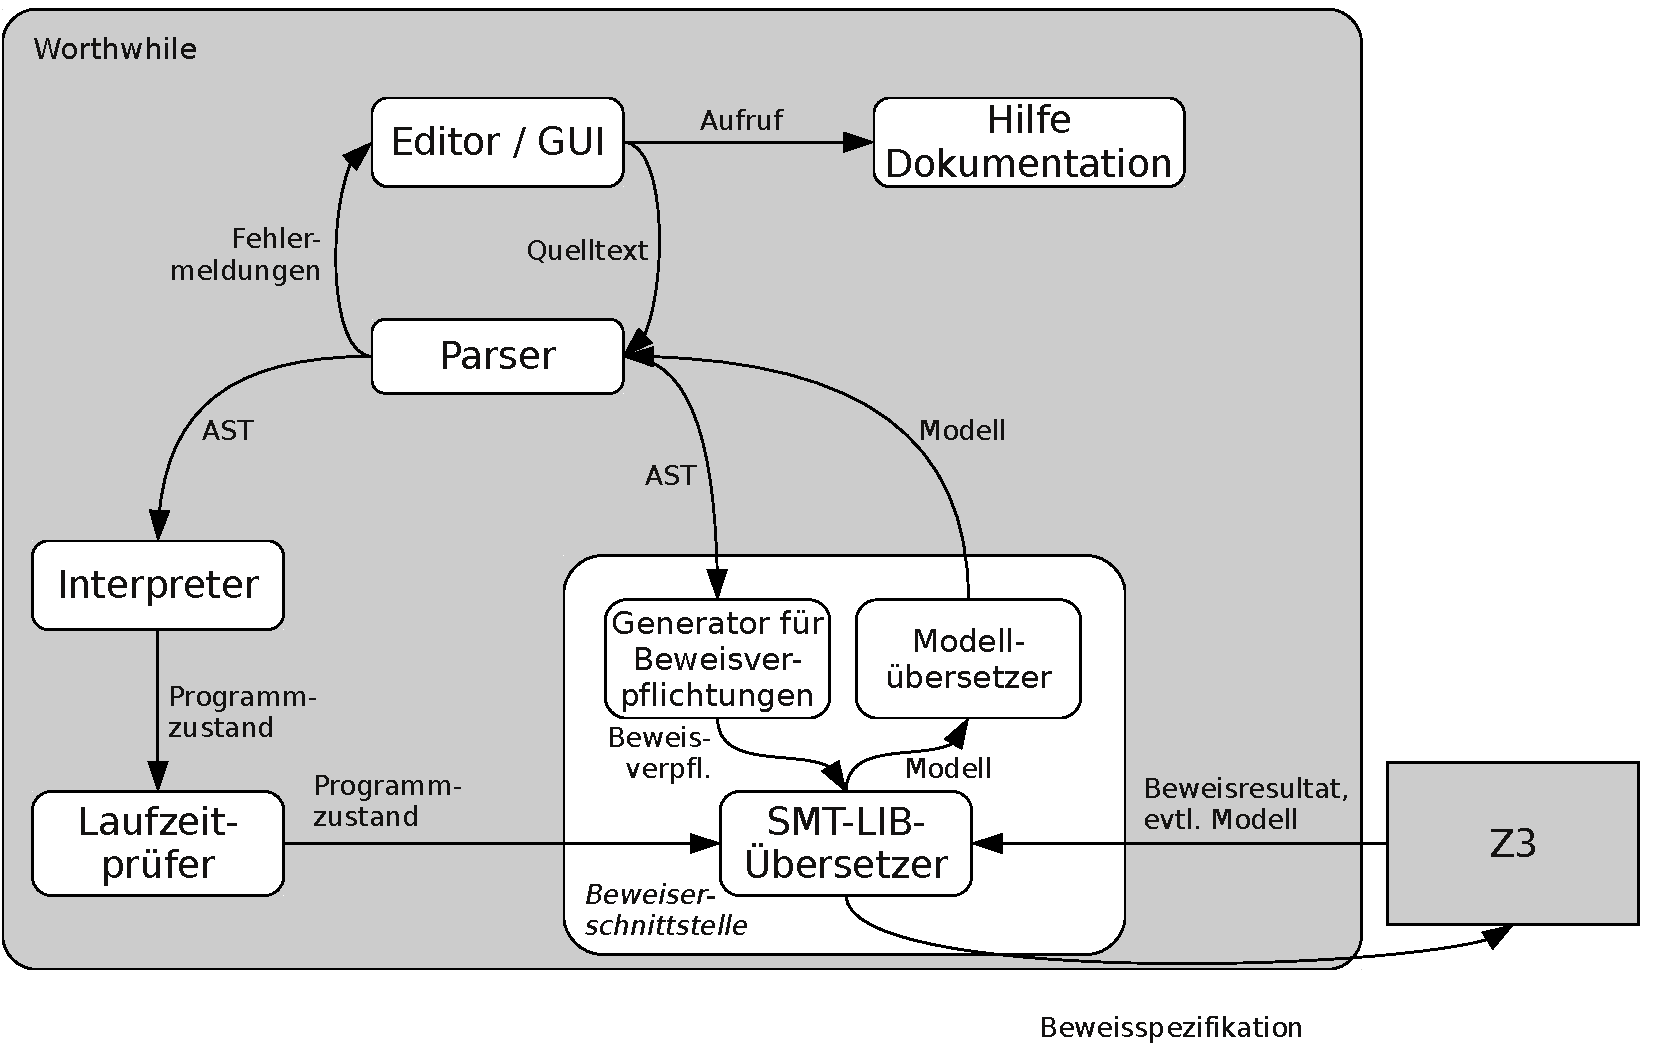
\includegraphics[width=\textwidth]{architektur/architektur.pdf}


\section{Produktleistungen}%

\begin{reqlist}{P}%
    \req{010}{Ansprechbarkeit der Benutzeroberfläche

    Während der Interpreter Code ausführt oder ein Analyseprozess läuft, bleibt die Benutzerschnittstelle ansprechbar.}%
    \req{020}{Genauigkeit von Interpreter-""Operationen

    Alle mathematischen und logischen Operationen werden vom Interpreter exakt und ohne Genauigkeitsverlust ausgeführt. Wenn dies nicht möglich ist, bricht der Interpreter mit einer Fehlermeldung ab.}%
\end{reqlist}%


\section{Weitere nichtfunktionale Anforderungen}%

\begin{description}%
    \item [Referenzplattform] Das Programm muss unter Verwendung der Oracle Java Runtime Environment in der Version 6 oder höher unter Linux alle Anforderungen erfüllen.
    \item [Lizenz von Z3] Die Lizenz des von Microsoft entwickelten Beweisers Z3 lässt nur nichtkommerzielle Nutzung zu. Eine kommerzielle Nutzung von \emph{Worthwhile} muss deshalb ausgeschlossen werden.
    \item [Austauschbarkeit des Beweisers] Obwohl das Programm für den Gebrauch mit dem Beweiser Z3 entwickelt wird, muss sich dieser trotzdem gegen andere Beweiser mit SMT-LIB-Schnittstelle austauschen lassen.
\end{description}


\section{Grafische Benutzeroberfläche (GUI)}

Die GUI bietet eine grafische Schnittstelle zur Steuerung aller Komponenten von Worthwhile. Während wichtige Komponenten wie Interpreter und Beweiser auch ohne die GUI ausgeführt werden können, erleichtert eine grafische Oberfläche das Arbeiten mit ihnen ungemein.

Die GUI enthält alle Funktionen, die man von einer modernen integrierten Entwicklungsumgebung erwartet. Dazu gehört insbesondere ein Editor mit Syntaxhervorhebung, Code Folding und Markierung von Parserfehlern während der Eingabe. Weiterhin bietet sie Funktionen zum Ausführen des Interpreters und des Beweisers sowie einen Debugger.

Die GUI benutzt das Entwurfsmuster \textit{Model-View-Controller.} Dabei ist der AST das Modell, das von diversen Sichten (Views) wie dem Editor, der Parserfehler-Ansicht oder dem Projektexplorer angezeigt wird. Über GUI-Befehle werden Änderungen am Modell ausgelöst, sodass die GUI selbst hier als Controller fungiert.

Weitere eingesetzte Entwurfsmuster sind \textit{Strategy} etwa bei der Bereitstellung von AutoEdits und bei den Provider"-klassen (\texttt{Label"-Provider}, \texttt{Quickfix"-Provider}, \texttt{Outline"-Tree"-Provider} etc.) sowie \textit{Plugin}, da die Worthwhile-Komponente in die existierende Eclipse-Plattform über Plugins eingebunden wird. Diese Plugins implementieren Schnittstellen, die durch die Plattform vorgegeben sind.

\subsection{Klassenentwurf}

\subsubsection{class WorthwhileEditor}

Der Editor dient zur Bearbeitung von Dateien vom Typ Worthwhile-Programm (Dateiendung \texttt{.ww}). Für jede geöffnete Datei erstellt die GUI eine neue Instanz dieser Klasse.

\begin{description}
	\method{public IResource getResource()} Gibt die vom Editor bearbeitete Ressource zurück. In diesem Fall ist dies eine Datei, also eine Instanz einer Klasse, die \texttt{IFile} implementiert.
	\method{public bool isEditable()} Gibt zurück, ob die im Editor geöffnete Datei zum aktuellen Zeitpunkt verändert werden kann.
\end{description}

\subsubsection{class WorthwhileLabelProvider}

Der Label Provider dient dazu, einem Sprachelement eine Beschriftung und ein Symbol zuzuweisen. Wo in der GUI eine textuelle Repräsentation eines Sprachelements angezeigt werden muss (etwa in Tooltips oder bei der Codevervollständigung), wird auf den \texttt{LabelProvider} zurückgegriffen.

\begin{description}
	\method{public String getText(element : EObject)} Gibt den Beschriftungstext für das Sprachelement \texttt{element} zurück.
	\method{public String getImage(element : EObject)} Gibt den Dateinamen eines Symbols für das Sprachelement \texttt{element} zurück.
\end{description}

\subsubsection{class WorthwhileDescriptionLabelProvider}

In manchen Fällen müssen Beschriftungstexte und Symbole für Sprachelemente angezeigt werden, ohne dass die entsprechende Datei geöffnet ist. Ein Beispiel dafür ist die Fehlerübersicht, in der alle Parserfehler der Dateien eines Projekts angezeigt werden, auch wenn die Datei nicht in einem Editor geöffnet ist. Dazu wird in einem internen Cache der GUI für jedes Sprachelement einer Datei eine sogenannte Beschreibung (\texttt{IEObjectDescription}) abgelegt. Der \texttt{DescriptionLabelProvider} dient dazu, aus einer solchen Beschreibung einen Beschriftungstext und ein Symbol zu extrahieren.

\begin{description}
	\method{public String getText(description : IEObjectDescription)} Gibt den Beschriftungstext für das durch \texttt{description} beschriebene Sprachelement zurück.
	\method{public String getImage(description : IEObjectDescription)} Gibt den Dateinamen eines Symbols für das durch \texttt{description} beschriebene Sprachelement zurück.
\end{description}

\subsubsection{class WorthwhileQuickfixProvider}

Da durch den \texttt{Validator} nicht nur syntaktische, sondern auch semantische Fehler erkannt werden sowie durch den \texttt{SyntaxErrorMessageProvider} die Art eines Syntaxfehlers näher spezifiert werden kann, ist es möglich, für bestimmte Fehler und Warnungen eine Reihe von Korrekturvorschlägen anzubieten. Der Benutzer kann einen dieser Korrekturvorschläge zur automatischen Anwendung auswählen.

Die in dieser Klasse spezifizierten Korrekturfunktionen erhalten als Parameter jeweils eine Fehlerbeschreibung (\texttt{Issue}) sowie eine Referenz auf einen \texttt{Issue"-Resolution"-Acceptor}, der die Korrekturvorschläge entgegennimmt und an die GUI weiterleitet.

\begin{description}
	\mlmethod{public void addFunctionReturnType(issue : Issue, \\ acceptor : IssueResolutionAcceptor)} Bietet für eine Funktion mit nicht spezifiziertem Rückgabetyp das Hinzufügen eines Rückgabetyps an.
	%\method{TODO}
\end{description}

\subsubsection{class WorthwhileOutlineTreeProvider}

Für größere Programmdateien ist es eine Hilfe, die in einem Programm vorkommenden Elemente wie Funktions- und Variablendeklarationen auf einen Blick zu sehen. Die GUI bietet diese Möglichkeit, indem im \textit{Outline}-Fenster eine hierarchische Ansicht des Programmtextes angezeigt wird. Diese Ansicht wird durch den \texttt{OutlineTreeProvider} erstellt.

\begin{description}
	\method{public IOutlineNode createRoot(document : IXtextDocument)} Erstellt den Wurzelknoten der hierarchischen Ansicht aus dem Dokument \texttt{document}.
	\method{public void createChildren(parent : IOutlineNode, modelElement : EObject)} Erstellt die Kindknoten des gegebenen Knotens \texttt{parent} in der Outline-Ansicht, wobei der Knoten \texttt{parent} das Sprachelement \texttt{modelElement} repräsentiert.
\end{description}

\subsubsection{class WorthwhileProposalProvider}

Für die Code-Vervollständigung muss eine Reihe von Vorschlägen erstellt werden. Während sich die meisten direkt aus der Grammatik und den schon vorhandenen AST-Elementen ableiten lassen, kann es wünschenswert sein, eigene Vorschläge zu erstellen oder vorhandene anzupassen. Diese Aufgabe übernimmt der \texttt{ProposalProvider}.

\begin{description}
	\mlmethod{public void complete\_$\{$RegelName$\}$(model : EObject, ruleCall : RuleCall, context~:~ContentAssistContext, acceptor~:~ICompletionProposalAcceptor)} Übergibt eine Liste von Vervollständigungs-Vorschlägen an das \texttt{acceptor}-Objekt, das sie an die GUI weiterleitet. Dabei ist \texttt{RegelName} die Regel aus der Sprachdefinition, für die Vorschläge erstellt werden sollen. Wird beispielsweise an der aktuellen Stelle im Programm gemäß Sprachspezifikation eine Zahl erwartet, so wird die Methode \texttt{complete\_{}NUMBER} aufgerufen.
	\mlmethod{public void complete$\{$TypName$\}$\_{}$\{$FeatureName$\}$(model~:~EObject, assignment~:~Assignment, context~:~ContentAssistContext, acceptor~:~ICompletionProposalAcceptor)}
	Übergibt eine Liste von Vervollständigungs-Vorschlägen an das \texttt{acceptor}-Objekt, das sie an die GUI weiterleitet. Dabei ist \texttt{TypName} der Typ des Sprachelements, für das ein Vorschlag erstellt werden soll, und \texttt{FeatureName} das spezifische Feature des Sprachelements (beispielsweise \texttt{completeFunctionDeclaration\_{}ReturnType}).
\end{description}

\subsubsection{class WorthwhileAutoEditStrategyProvider}

Mit "`AutoEdit"' wird die Funktion bezeichnet, eine Eingabe im Texteditor abzufangen und je nach Inhalt Aktionen im Texteditor auszulösen. Dazu gehört das automatische Schließen geöffneter Klammern ebenso wie die Umwandlung von Operatorenzeichen in textueller Repräsentation (siehe \ref{textrep}) in die entsprechenden Unicode-Operatorenzeichen.

\begin{description}
	\mlmethod{public List<IAutoEditStrategy> getStrategies(sourceViewer~:~ISourceViewer, contentType~:~String)}
	Gibt eine Liste von AutoEdit-Strategien für den gegebenen Quelltexteditor und den gegebenen Inhaltstyp zurück.
\end{description}


\section{Qualitätsanforderungen}%

\begin{reqlist}{Q}%
    \req{01}{Abbruch durch den Interpreter}{Der Interpreter darf einen Programmdurchlauf nicht von sich aus abbrechen, ohne eine ausführliche Fehlermeldung anzuzeigen.}
    \req{02}{Dokumentationsgrad}{Zu jedem Schlüsselwort oder Syntaxelement der WHILE-Sprache existiert eine eigene Dokumentationsseite, auf der die Funktionsweise erklärt und anhand mindestens eines Beispielprogramms veranschaulicht wird.}
	\req{03}{Korrektheit des Analysewerkzeugs (I)}{Ein vom Analysewerkzeug als korrekt eingestuftes Programm muss auf jeden Fall korrekt sein.}
    \req{04}{Korrektheit des Analysewerkzeugs (II)}{Ein vom Analysewerkzeug als inkorrekt eingestuftes Programm muss auf jeden Fall inkorrekt sein.}
    \req{05}{Korrektheit des Analysewerkzeugs (III)}{Falls ein Programm weder als korrekt noch als inkorrekt vom Analysewerkzeug eingestuft werden kann, muss das Werkzeug eine entsprechende Fehlermeldung ausgeben. Das Programm darf in diesem Fall jedoch keinesfalls als inkorrekt eingestuft werden.}
    \req{06}{Beweiserabbruch}{Dass gerade der Beweiser ausgeführt wird, muss dem Benutzer angezeigt werden und der Benutzer muss die Möglichkeit haben, die Ausführung des Beweisers abzubrechen. Dabei geht es insbesondere um die Behandlung von Fällen, in denen der Beweiser unbestimmt lange läuft und unbekannt ist, ob er zu einer Entscheidung kommt.}%
    \req{07}{Gegenbeispielanzeige}{Im Idealfall müssen Modelle, die der Beweiser bei der Nichterfülltheit einer Spezifikation liefert, im Quelltext auf den fehlerhaften Codeabschnitt zurückgeführt werden. Unter allen Umständen muss derjenige Teil der Spezifikation~(eine Formel in den Annotationen) markiert werden, für welche der Beweiser ein Gegenbeispiel gefunden hat, und das zurückgelieferte Modell muss in der WHILE-Sprache (Belegungen der deklarierten Variablen bzw. Parameter, Funktionsdefinitionen) angezeigt werden.}%
    \req{08}{Unabhängigkeit von Programmdurchläufen}{Mehrere Programmdurchläufe, die gleichzeitig oder nacheinander ablaufen, beeinflussen einander nicht. Mehrere verschiedene Durchläufe ein und desselben Programms erzeugen bei gleicher Eingabe jederzeit dieselbe Ausgabe.}
\end{reqlist}


\section{Globale Testfälle und Testszenarien}

\begin{reqlist}{T}
	\req{01}{Randfälle korrekter Programme}{
		\testspec
		{Korrektes Verhalten des Parsers, Interpreters und Beweisers bei Programmen, die der Sprachspezifikation entsprechen, aber gewisse Randfälle darstellen.}
		{Die Entwicklungsumgebung ist gestartet, kein Programm ist geladen}
		{
			\begin{enumerate}
				\item Öffnen des Testprogramms:
					\begin{reqlist}{T}
						\req{01a}{Leeres Programm}{Das leere Programm, d.h. die Datei enthält keine Anweisungen (aber eventuell Leerzeilen)}
						\req{01b}{Verschachteltes Programm}{Ein Testprogramm mit verschachtelten Schleifen und If-Abfragen bis zu einer Schachtelungstiefe von 1000. Die Abfragen und Schleifen sind so gestaltet, dass alle Anweisungen erreichbar sind. Das Programm enthält keine Zusicherungen.}
						\req{01c}{Langes Programm}{Ein Testprogramm ohne If-Abfragen, Schleifen und Zusicherungen, aber mit mehr als 10.000 Anweisungszeilen.}
					\end{reqlist}
				\item Ausführen des Programms durch entsprechenden Befehl
				\item Verifizieren des Programms durch entsprechenden Befehl
			\end{enumerate}
		}
		{
			\begin{enumerate}
				\item Der Interpreter wird ohne Fehlermeldung beendet.
				\item Das Verifizieren des Programms schlägt nicht fehl (entweder wird Erfolg zurückgemeldet oder eine Warnung wegen fehlender Zusicherungen ausgegeben).
			\end{enumerate}	
		}
	}
	
	\req{02}{Fehlerhafte Programme}{
		\testspec
		{Korrektes Verhalten des Parsers, Interpreters und Beweisers bei Programmen, die nicht der Sprachspezifikation entsprechen}
		{Die Entwicklungsumgebung ist gestartet, kein Programm ist geladen}
		{
			\begin{enumerate}
				\item Öffnen des Testprogramms:
					\begin{reqlist}{T}
						\req{02a}{Falsch geschriebene/nicht existierende Schlüsselwörter}{Es werden in einem korrekten Programm Schlüsselwörter gegen andere Wörter, die keine Schlüsselwörter sind, ausgetauscht.}
						\req{02b}{Fehlender Leerraum}{Es werden in einem korrekten Programm Leerzeichen gelöscht, sodass das resultierende Programm nicht mehr der Sprachspezifikation entspricht.}
						\req{02c}{Fehlende/überflüssige Operanden}{Es wird eine binäre mathematische oder logische Operation mit nur einem Operanden oder eine unäre mathematische oder logische Operation mit zwei Operanden aufgerufen.}
						\req{02d}{Operanden vom falschen Typ}{Es wird eine mathematische oder logische Operation mit Operanden aufgerufen, die nicht dem von der Operation geforderten Typ entsprechen.}
						\req{02e}{Ungültige Parameter bei Methodenaufruf}{In einem Methodenaufruf werden Parameter übergeben, die in Anzahl und/oder Typ nicht der Methodensignatur entsprechen.}	
						\req{02f}{Fehlerhafter Methodenaufruf}{Es wird versucht, eine nicht deklarierte Methode aufzurufen.}
						\req{02g}{Verwenden nicht deklarierter Variablen}{Es wird versucht, eine Variable zu verwenden, die nicht deklariert wurde. \\ \emph{Dieser Testfall findet nur Anwendung, wenn die Sprachspezifikation das Deklarieren der Variablen vor ihrer Verwendung vorschreibt.}}
						\req{02h}{Unerlaubte Typkonvertierung}{Es wird versucht, einer Variable einen Wert zuzuweisen, der nicht ihrem Typ entspricht. \\ \emph{Dieser Testfall findet nur Anwendung, wenn die Sprachspezifikation eine automatische Typkonvertierung von Variablen nicht erlaubt.}}
					\end{reqlist}
				\item Ausführen des Programms durch entsprechenden Befehl
				\item Verifizieren des Programms durch entsprechenden Befehl
			\end{enumerate}
		}
		{
			\begin{enumerate}
				\item Die fehlerhafte Stelle wird im Editorfenster markiert.
				\item In der Fehlerliste wird eine Fehlerbeschreibung angezeigt.
				\item Durch Doppelklick auf den Eintrag in der Fehlerliste springt der Cursor an die fehlerhafte Stelle im Programm
				\item Beim Versuch, das Programm auszuführen, wird eine (allgemeine oder spezifische) Fehlermeldung ausgegeben.
				\item Beim Versuch, das Programm zu verifizieren, wird eine (allgemeine oder spezifische) Fehlermeldung ausgegeben.
			\end{enumerate}	
		}
	}
	
	\req{03}{Syntaxhervorhebung im Editor}{
		\testspec{Korrekte Syntaxhervorhebung im Editor}
		{keine}
		{\begin{enumerate}
			\item Es wird ein Programm geladen, das alle definierten Sprachkonstrukte mindestens einmal enthält.
		\end{enumerate}}
		{
		\begin{enumerate}
			\item Es werden alle in der Sprache definierten Elemente (Schlüsselwörter, Funktions- und Variablennamen, Kommentare, Zahlen) gemäß den Einstellungen in der Entwicklungsumgebung hervorgehoben.
		\end{enumerate}
		}
	}
	
	\req{04}{Debuggen eines Programms}{
		\testspec{Korrektes Verhalten des Interpreters bei Ausführung der Debug-Operationen}
		{Es ist ein Programm geladen, das der Sprachspezifikation entspricht und alle definierten Sprachkonstrukte mindestens einmal enthält.}
		{\begin{enumerate}
			\item Mittels des entsprechenden Befehls in der Entwicklungsumgebung werden ein oder mehrere Haltepunkte gesetzt.
			\item Der Interpreter wird über den entsprechenden Befehl im Debug-Modus gestartet.
			\item Nach Anhalten des Programms am Breakpoint werden mehrmals hintereinander der Einzelschritt-Befehl und der Überspringen-Befehl ausgeführt. Dabei sollen beide Befehle auch in Zeilen ausgeführt werden, in denen sich Methodenaufrufe befinden.
			\item Es wird einer der folgenden Schritte ausgeführt (der Testfall muss zweimal durchgeführt werden, damit beide Schritte abgedeckt werden):
			\begin{enumerate}
			\item Der Programmablauf wird durch entsprechenden Befehl abgebrochen.
			\item Der Programmablauf wird durch entsprechenden Befehl fortgesetzt.			
			\end{enumerate}
			\item Wie oben, allerdings wird der Interpreter im Ausführungsmodus gestartet.
		\end{enumerate}}
		{\begin{enumerate}
			\item Die Haltepunkte werden im Editor und in der Haltepunktübersicht angezeigt.
			\item Nach Ausführen des Programms im Debug-Modus hält der Interpreter vor der Zeile, die den ersten Haltepunkt enthält.
			\item Bei Ausführung des Einzelschritt-Befehls führt der Interpreter den nächsten Befehl aus, wobei er in Methodenaufrufe hineinspringt.
			\item Bei Ausführung des Überspringen-Befehls führt der Interpreter den nächsten Befehl aus, wobei er nicht in Methodenaufrufe springt.
			\item Bei Ausführung des Abbruchbefehls wird der Programmablauf sofort abgebrochen.
			\item Bei Ausführung des Fortsetzen-Befehls führt der Interpreter das Programm bis zum nächsten Haltepunkt bzw. bis zum Programmende aus.
			\item Nach Ausführen des Programms im Ausführungsmodus ignoriert der Interpreter die Haltepunkte und führt das Programm bis zum Ende aus.
			\item Bei Ausführung im Debug- und Ausführungsmodus verhält sich das Programm gleich (beispielsweise in Bezug auf Terminierung des Programmablaufs).
		\end{enumerate}}
	}
	
	\req{05}{Ansprechbarkeit der Benutzeroberfläche}{
		\testspec{Ansprechbarkeit der Benutzeroberfläche bei Ausführung eines Programms}
		{Es ist ein Programm geladen, das der Sprachspezifikation entspricht und eine Endlosschleife enthält.}
		{\begin{enumerate}
			\item Der Benutzer startet den Interpreter.	
			\item Während der Interpreter läuft, bricht der Benutzer das Programm durch entsprechenden Befehl ab.
		\end{enumerate}}
		{\begin{enumerate}
			\item Der Interpreter reagiert in weniger als einer Sekunde auf den Befehl und bricht das Programm ab.
		\end{enumerate}}
	}
	
	\req{06}{Ändern von Variablenwerten während des Programmablaufs}{
		\testspec{Korrekte Auswirkung der Änderung von Variablenwerten}
		{Es ist ein Programm geladen; mehrere Haltepunkte sind im Programm gesetzt.}
		{\begin{enumerate}
			\item Der Benutzer startet den Interpreter im Debug-Modus.	
			\item Nach Halt des Interpreters gibt der Benutzer im Fenster zur Ausdrucksauswertung einige Ausdrücke ein, darunter sowohl gültige als auch ungültige (Syntaxfehler, nicht deklarierte Variablen etc.).
			\item Der Benutzer ändert im Variablenfenster die Werte von Variablen so, dass der Programmablauf dadurch beeinflusst wird (beispielsweise: Schleife wird abgebrochen).
			\item Der Benutzer setzt die Programmausführung fort.
		\end{enumerate}}
		{\begin{enumerate}
			\item Die Ausdrücke werden korrekt ausgewertet; für nicht auswertbare Ausdrücke wird eine aussagekräftige Fehlermeldung angezeigt.
			\item Nach Änderung der Variablenwerte werden die Werte der Ausdrücke im Ausdrucksfenster aktualisiert.
			\item Beim Fortsetzen der Programmausführung werden die neuen Variablenwerte übernommen und das Programm entsprechend ausgeführt.
		\end{enumerate}}
	}
	
\end{reqlist}

==== Für die GUI ====

  - alle Optionseinstellungen überprüfen
  - korrekte Speicherung der Optionseinstellungen überprüfen

==== Für das Verbindungsmodul zum Beweiser (statische Analyse) ====
  - Ein Programm mit allen Annotationen
  - Verschachtelte Schleifen
  - Rekursion
  - Funktionsaufrufe in Annotationen

\section{Spezielle Anforderungen an die Entwicklungsumgebung}%

\begin{description}%
    \item [Teamkommunikation] Wiki~(intern), E-Post-Verteiler~(intern), \href{http://xmpp.org/extensions/xep-0045.html}{XMPP Multi-User Chat}
    \item [Dokumentenerstellung] \LaTeX{}%
    \item [Entwurf] Ein Programm zur Visualisierung der Programmstruktur
    \item [Versionskontrolle] git%
    \item [Entwicklungsumgebung] Eclipse%
    \item [Validierung] Ein Testing Framework sowie ein \see{Continous Integration} Server, um eine Test-Driven-Development-ähnliche Vorgehensweise bei der Entwicklung zu fördern
\end{description}%


\section{Zeit- und Ressourcenplanung}%

\subsection{Implementierungsaufwand}%

\begin{figure}[H]
  \begin{tabular}{| l | l | l | }
    \hline
    \textbf{Modul} & \textbf{Aufwand (h)}\\ \hline
    \see{Parser} & 25\\ \hline
    \see{Interpreter} & 70 \\ \hline
    \see{Run-time-checker} & 70\\ \hline
    Schnittstelle zum \see{Beweiser} & 90 \\ \hline
    Grafische Benutzeroberfläche & 40 \\ \hline
    Dokumentation & 20 \\ \hline
    Beispielsammlung & 15\\ \hline
    Unit- und GUI-Tests & 20 \\ \hline \hline
    \textbf{Gesamt} & 350 \\ \hline
  \end{tabular}
\end{figure}

\subsection{Gesamtaufwand}%

Die gesamte zur Verfügung stehende Arbeitszeit beträgt geschätzte 290~Arbeitsstunden pro Person, insgesamt also 1740~Personenarbeitsstunden.

Die Arbeitszeit pro Person berechnet sich wie folgt aus den Leistungspunkten~(LP) für die PSE-Veranstaltung: $30\textrm{h}/\textrm{LP} \cdot 8~\textrm{LP} \cdot 1,2$~(aufgerundet).

\subsection{Phasenverantwortliche}%

\begin{tabular}{| l | l | }
    \hline
    \textbf{Phase} & \textbf{Verantwortlicher} \\ \hline
    Pflichtenheft & Chris Hiatt \\ \hline
    Entwurf & Joachim Priesner \\ \hline
    Implementierung & Stefan Orf, Matthias Wagner \\ \hline
    Qualitätssicherung & Leon Handreke \\ \hline
    Abnahme/Abschlusspräsentation & Fabian Ruch \\ \hline
\end{tabular}

\subsection{Ressourcen}%

\begin{itemize}%
    \item Rechner, der die Mindestanforderungen erfüllt
\end{itemize}%


\clearpage
\appendix

\section{Glossar}

% TODO: alphabetisch sortieren (wenn Glossar fertig)

\begin{description}
    \item[Befehl~(GUI)] Aktion, die der Benutzer durch Aufruf eines Menüeintrags, Anklicken einer Schaltfläche oder Betätigung einer Tastenkombination auslösen kann.
    \item[Programm] Folge von Anweisungen formuliert nach den Regeln einer Programmiersprache, die vom Computer ausgeführt werden können.
    \item[Programmzustand] Eindeutige Beschreibung des Zustandes eines in Ausführung befindlichen Programms, bestehend aus Anweisungszeiger, Aufrufstack und Variablenwerten.
    \item[Parser] Programm, das aus einem Quelltext in Textform eine maschinenlesbare Repräsentation dieses Quelltextes erstellt.
    \item[Interpreter] Ein Programm, welches Anweisungen in maschinenlesbarer Quelltextform in Anweisungen für den Computer umsetzt und diese ausführt.
    \item[Run-time checker] Eine Komponente der Laufzeitumgebung, der zur Laufzeit das Zutreffen der Zusicherungen auf den Programmzustand überprüft und eventuelle Fehler meldet.
    \item[Beweiser] Ein Programm, mit dessen Hilfe man die Gültigkeit von Zusicherungen für ein Programm für alle Programmeingaben beweisen kann.
    \item[Zusicherung] Anforderung an den Programmzustand, die an einer oder mehreren festgelegten Stellen im Programmablauf gelten muss.
    \item[Annotation] Syntaxelement einer Programmiersprache, das selbst nicht vom Interpreter ausgeführt wird, sondern zusätzliche Informationen über ein anderes Syntaxelement (eventuell für ein externes System) bereitstellt.
    %\item[Beweisverpflichtung] TODO: What is this?
    \item[Prädikatenlogik] Ein logisches System, das es erlaubt, mathematische Aussagen zu formalisieren und auf Gültigkeit zu überprüfen. %First-order, Second-order
    \item[WHILE-Sprache (Interpreter)] Einfache Programmiersprache, in der nur simple Syntaxkonstrukte wie z.~B.\ eine \texttt{while}-Schleife verfügbar sind.
    \item[Annotationssprache (Beweiser)] Eine Sprache, in der \see Zusicherungen formuliert werden. Sie kann als eine Annotation direkt an der passenden Stelle eines Programms eingefügt werden.
    \item[Schleifeninvariante] Aussage, die beim Eintritt in einer Schleife, bei jedem Schleifendurchlauf und beim Verlassen der Schleife erfüllt ist.
    \item[Gültigkeitsbereich] Eindeutig umgrenzter Bereich in einem Programmcode, beispielsweise der Rumpf einer Schleife oder einer Methode. Auf eine dort deklarierte Variable oder Annahme kann nur in diesem Bereich Bezug genommen werden.
    \item[Zusicherungensprache (Run-time checker)] Eine Sprache in der \see Zusicherungen für den \see Run-time checker formuliert sind.
    \item[SMTLIB2~(Satisfiability Modulo Theories Library)] Format zur Spezifikation von prädikatenlogischen Formeln zwecks Überprüfung auf Erfüllbarkeit, erstellt von der gleichnamigen Initiative
    \item[Z3] Von Microsoft Research entwickeltes Computerprogramm zur Erfüllbarkeitsüberprüfung prädikatenlogischer Formeln
    \item[Eclipse] Java-Entwicklungsumgebung basierend auf einer leicht erweiterbaren Plugin-Architektur.
\end{description}



\end{document}
